%\subsection{Weighted Sum Solution}
%\label{sec:algo_weightedsum}
%
%As our problem is a multi-objective programming problem, we can solve it by a Weighted Sum Solution. A weight $w$ which demonstrates the optimization preference to \textbf{Coverage} and \textbf{Overlap} is first given by the decision maker. So the problem can be reformulated to a single-objective problem and is formalized as follow, we call it AC-QP.
%\begin{eqnarray}
%\min_{x} && (1-w)x^TPx-wd^Tx \label{eq:objfunc}\\
%\rm{subject~to} && x_s(x_s-1)=0\\
%&&\sum_{s\in S}{x_s}=k
%\end{eqnarray}
%
%In the definition above, the equation $x_s(x_s-1)=0$ is non-convex quadratic constraint, so the problem is a case of non-convex QCQR.
%
%Then the equivalent SDP(semidefinite programming) formulation of AC-QP can be indicated as following, we call it AC-SDP.
%\begin{eqnarray}
%\min_{X,x} && Q\bullet X+c^Tx \label{qcqpsubj}\\
%\rm{subject~to} && e^Tx=k\\
%&&diag(X)=x\\
%&&X=xx^T
%\end{eqnarray}
%where $Q\bullet X=trace(QX)=\sum\limits^n_{i=1}\sum\limits^n_{j=1}{Q_{ij}X_{ij}}$ and $Q=(1-w)P, c=-wd$.
%
%Because we have nonconvex constraints in AC-SDP, so $X=xx^T$ is relaxed to $X-xx^T\succeq 0$. And then the semidefinite relaxation of AC-QP is obtained as following, we call it AC-SDR.
%\begin{eqnarray}
%\min_{X,x} && Q\bullet X+c^Tx \\
%\rm{subject~to} && e^Tx=k\\
%&&diag(X)=x\\
%&&\left[
%\begin{array}{cc}
%1 & x^T\\
%x & X
%\end{array}
%\right]\succeq 0
%\end{eqnarray}

%\subsection{Quadratic Convex Reformulation}
%Since our problem has non-convex constraints, we use a \emph{Quadratic Convex Reformulation} (QCR)
%to reformulate the problem to a convex one. This method apply a continuous relaxation to the 0-1
%constraint, i.e., we weaken the 0-1 constraint to $0\leq x_i \leq 1$. After continuous relaxation,
%we need to reformulate the original problem to make the lower bound of continuous relaxation equal
%to the lower bound of Semi-Definite Program relaxation. Suppose strong duality holds for the SDP relaxation
%and a dual optimal solution ($\lambda^*, \mu^*$) exists, if we perturb the objective function
%\ref{qcqpsubj} by:
%\begin{itemize}
%\item adding $x^Tdiag(\lambda^*)x-(\lambda^*)^Tx$ and $\mu^*(e^Tx-k)$
%\item changing the equality constraints to inequality constraints with opposite sign,
%\end{itemize}
%then the reformulated problem is convex and the lower bound of the continuous relaxation equals to
%the lower bound of SDP relaxation. The reformulated problem is shown as follows:
%\begin{eqnarray}
%\min_{x} && (1-w)x^TPx-wd^Tx \nonumber \\
%&&+x^Tdiag(\lambda^*)x-(\lambda^*)^Tx \nonumber\\
%&&+\mu^*(e^Tx-k) \\
%\rm{subject~to} && e^Tx\leq k\\
%&& e^Tx\geq k\\
%&& 0\leq x_s \leq 1, for all s\in S
%\end{eqnarray}

\subsection{Graph Based Approach}
\begin{eqnarray*}
\max_{x} && \sum_{s\in S}{Coverage(s)\cdot x_s} \\
\rm{subject~to} && x_s\cdot (x_s-1)=0\\
&&\sum_{s\in S}{x_s}=k\\
&& Overlap(s,t)\cdot x_t\cdot x_s\leq \tau, for\ all\ s,t\in S, s\neq t
\end{eqnarray*}

\subsubsection{Graph Representation}
Let us consider the following graph representation of a set $S$ of concepts. Let $G_{S,\tau}=(V,E)$ be an undirected graph such that there is a vertex $v_i\in V$ for each concept $s_i\in S$ with the weight $w(v_i)=Coverage(s_i)$ and an edge $(v_i,v_j)\in E$, if and only if, $Overlap(s_i,s_j)\leq \tau$ for the corresponding concepts $s_i,s_j,s_i\neq s_j$. An example is shown in \figref{fig:graph_model}.
\begin{figure}[th]
\centering
\epsfig{file=figure/graph_model.eps,width=1.0\columnwidth}
\caption{(a) Concept set $S$ with overlap constraint $\tau$ as the radius and (b) the corresponding graph representation $G_{S,\tau}$}
\label{fig:graph_model}
\end{figure}

Let us recall a couple of graph-related definitions. A \emph{complete subgraph} $D$ in a graph $G$ is a subgraph of $G$ such that every two vertices in $D$ are joined by an edge. And a \emph{maximum complete subgraph} is such a subgraph of $G$ with the maximum sum of vertices weight.

Considering the definition of \emph{action conceptualization} problem, solving such problem is equivalent to finding a \emph{maximum complete subgraph} with $k$ vertices in the corresponding graph  $G_{S,\tau}$, we call it \emph{graph based action conceptualization} problem.

\subsubsection{Backtracking Method}
In this section, we will give a graph search algorithm to solve \emph{graph based action conceptualization} problem we have proposed.
Backtracking is a general algorithm for finding all (or some) solutions to some computational problem, that incrementally builds candidates to the solutions, and abandons each partial candidate $c$ ("backtracks") as soon as it determines that $c$ cannot possibly be completed to a valid solution.
\begin{figure}[th]
\centering
\epsfig{file=figure/search_tree.eps,width=0.8\columnwidth}
\caption{A snapshot of the actual search tree for the example graph in \figref{fig:graph_model} with constraint $k=3$}
\label{fig:search_tree}
\end{figure}
